\section{\name Construction}
\red{In this section, we present our \name construction, by starting with algorithms to build and update our proof index, and then detailed algorithms of our verification mechanism.}
%Then we use a highlevel {\it Verify} algorithm to introduce the flow of our algorithms in the following part.....organize}
%In particular, the algorithms ensure that \name can defend against the data integrity attacks and the replay attacks.}

\subsection{Building Proof Index}
%We now introduce how to build and update our proof index based on the MPT.
%\noindent\textbf{Initialization:} In the very beginning,
Algorithm~\ref{alg:Init} shows the pseudo-code of building the proof index and the authenticator (i.e., the {\it Init} algorithm defined in Definition~\ref{def:name}).
%\blue{Note that this algorithm only contains how to build the proof index, i.e., $Init(K_1,K_2, \mathcal{D}) \rightarrow \{\lambda\}$. The generation of the authenticator $\pi$ by using symmetric key $K_3$ will be described later.}
It builds a proof index with MPT structure based on the document set $\mathcal{D}$, and the inverted index $\Delta$ computed from $\mathcal{D}$, where an inverted index refers to the index \red{that} indicates the documents containing a specific keyword.
%in the SSE initialization process.
For every keyword $w_i$ in the inverted list $\Delta$, we compute the key-value pairs which will be stored in our proof index, i.e., the MPT, where the key is the token of the distinct keyword $w_i$ and the value is the incremental hash of all the documents which contain the keyword. \blue{Note that, the \red{key stores} on the path of the tree and the value stores on the corresponding leaf node.}%In later subsections, we will use the root of the MPT to verify search results.
%which will play an important role in preventing the data integrity attack,
\begin{algorithm}[t]
  \caption{$Init$}
  \label{alg:Init}
  \begin{algorithmic}[1]
    \REQUIRE ~~\\{$K_1,K_2,K_3$: the symmetric keys; \blue{$ssk$: the secret key for signing;} $\mathcal{D}$: the document set;  $F, G: \{0, 1\}^k \times \{0, 1\}^* \rightarrow \{0, 1\}^*$ the pseudo-random functions; $IH: \{0, 1\}^* \rightarrow \{0, 1\}^k$ the incremental hash functions; $H: \{0, 1\}^* \rightarrow \{0, 1\}^k$ the hash function.}
    \ENSURE ~~\\{$\lambda$: the proof index established using the MPT;
                 $\pi$: the authenticator}
              \FOR {each $w_i \in \Delta$, where $\Delta$ is the inverted index which consists of $<w_i, D_{w_i}>$ pairs}
                \STATE{$\tau_{w_i} = F_{K_1}(w_i)$}
                \STATE{$V_{w_i} = \sum_{f_i \in D_{w_i}}IH (G_{K_2} (f_i))$}
                \STATE{$\lambda = \lambda.Insert (\tau_{w_i},V_{w_i})$}
              \ENDFOR
              \STATE{\blue{Generate authenticator $\pi$ as Equation (1) with symmetric key $K_3$ and secret key $ssk$.}\footnote{\blue{The detailed explanation on the authenticator $\pi$ will be described in Section~5.3.}}}
              \RETURN $\{\lambda,\pi\}$
  \end{algorithmic}
\end{algorithm}


The {\it Update} algorithm (see Definition~\ref{def:name}) updates the proof index on the server \red{and} supports three operations, i.e., the $add$, $delete$ and $edit$ operations. Here, the $edit$ operation is equivalent to adding a new file after deleting an old file. We briefly describe the algorithm here.  First, for $add$ operations, update tokens $\tau_u$ is split into the $\{\tau_{w_i}, G_{K_2} (f)\}$ pairs, where $\tau_{w_i}$ is the token of a specific keyword extracted from the file $f$ and $G_{K_2} (f)$ is a pseudo-random string of $f$. We locate the corresponding leaf nodes based on its tokens and add the value $IH (G_{K_2} (f))$ to the existing node value. A new leaf node will be created if a token does not have a corresponding leaf node. The $delete$ operation is similar to the $add$ operation. We locate the leaf node and subtract $IH (G_{K_2} (f))$ from the value of the leaf node. Note that the {\it PreUpdate} algorithm performed by the data owner provides the tokens for the {\it Update} algorithm conducted on the server.
%The {\it PreUpdate} algorithm is similar to the {\it Update} algorithm except that the data owner can see the plaintext of its data while the server can only see the ciphertext. Here, we do not duplicate the algorithms here.

\subsection{Verifying Search Results}
\begin{algorithm}[t]
  \caption{Verify}
  \label{alg:verification}
  \begin{algorithmic}[1]
    \REQUIRE {$K_1,K_2,K_3$: symmetric keys; \blue{$spk$: the public key for verifying signature;} $C_{w}$: the search results; $\rho$: the proof of the search results; $\tau_{w}$: the challenge made by the user; $\pi^t_q$: the authenticator received in the query time $t$; $\pi_c$:  the authenticator received in the checkpoint;}
    \ENSURE {$b \in \{0,1\}$, if $b = 1$, accept; otherwise, reject.}
          \STATE {$b \leftarrow Check (K_3,\blue{spk}, \pi^t_q, \pi_c)$}
          %\IF{$b_1=1$}K_1,K_2,K_3,C_w,\rho,\tau_{w},\pi^t_q
          \RETURN {$b \leftarrow b\quad  \&\&\quad Generate(K_1,K_2,K_3,C_w,\rho,\tau_{w},\pi^t_q)$}

          %\ELSE
          %  \RETURN {$reject$}
          %\ENDIF
  \end{algorithmic}
\end{algorithm}
Algorithm~\ref{alg:verification} shows the search result verification algorithm performed by data users (i.e., {\it Verify} algorithm shown in Definition~\ref{def:name}). Firstly, it checks the correctness of the authenticator by the {\it Check} algorithm.
% that implements a timestamp-chain based mechanism.
Here, an authenticator is used to ensure the freshness of the root. %If verification is not under the replay attacks,
If the authenticator is not replayed by the server, which means the root is fresh, then we use the {\it Generate} algorithm to verify search results by leveraging the root hash value extracted from the authenticator and the proof retrieved from the server. Finally, according to the results of {\it Check} and {\it Generate}, the algorithm can determine the freshness and integrity of the search results. In the later subsections, we will elaborate the {\it Check} and {\it Generate} algorithms.

%the tree root $rt$ according to the proof $\rho$ and $D_{w}$ that is the search result of SSE such that we can compare $rt$ with the root decrypted from the authenticator $\pi^t_q$ that is received at the query time $t$. The rebuild procedure prevents the data users from the data integrity attacks. According to the check and rebuild results, the algorithm decides if the users receive correct search results. In the later subsections, we will elaborate the {\it Check} and {\it Rebuild} algorithms.}



\subsection{Verifying Authenticators}
%{\bf The replay-proof mechanism in \name (ensures replay-proof authenticators ??)used in
In order to prevent cloud services from replaying previous authenticators and ensure the freshness of the root, we maintain a timestamp-chain for authenticators\red{, such that} users can trace authenticators in the chain and identify if the root is fresh. %, which is important to ensure the correctness of search verification.
Here, the timestamp-chain scheme is different from the timestamp mechanism used in SSE~\cite{stefanov2014practical}. Their schemes can only prevent servers from constructing data freshness attacks under the two-party model when the user holds the update information. Unfortunately, it may not be able to detect data freshness attack \red{in our concerned three-party model}. We show the details of our scheme below.%}
%which will be explain in detail in the following part. \name allows users to trace back the timestamp chain and verify if a search result is replayed.}
%, we cannot directly compare timestamps in authenticators.  the mechanism can correctly verify if
%To prevent such attacks,

  \begin{figure}[htb]
    \centering
    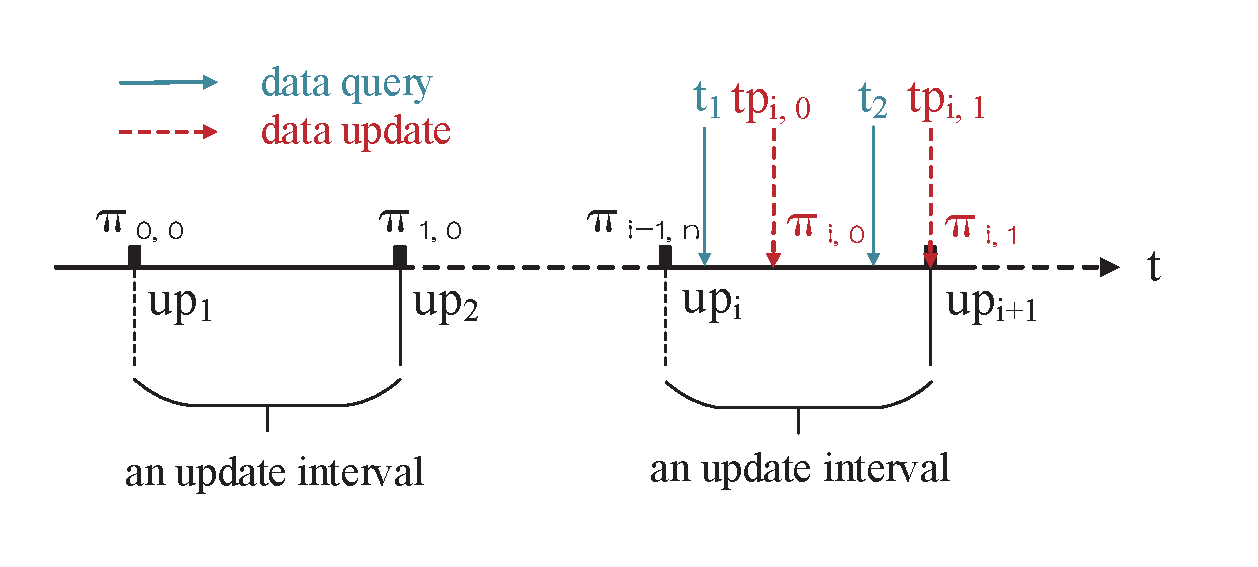
\includegraphics[width=3.5 in]{timestamp}
    \DeclareGraphicsExtensions.
    \caption{An illustration of the timestamp-chain mechanism}
    \label{fig:timestamp}
  \end{figure}

Firstly, we will show how the data owner creates the authenticator by leveraging the timestamp-chain. In the very beginning, a data owner sets an interval for authenticator update\footnote{In the performance evaluation section, i.e., Section~\ref{sec:experiments}, we will show the relationship between the update interval and the delays of detecting data freshness attacks.}, and then the fixed update time points are set to be $\{up_1, up_2, \cdots, up_i, \cdots, up_m\}$ (see Fig.~\ref{fig:timestamp}). %{\bf Here, we assume that the clock of the data owner, the data users and the cloud server is synchronized via Netword Time Protocol (NTP)~\cite{mills1991internet, mills2010network}. Some researches~\cite{kopetz1987clock, elson2002fine, zhou2007accurate} shows that the current clock synchronization accuracy can reach a few milliseconds or even tens of microseconds.}% and the network latency of them is almost the same.%The time slot between the two update points is called the update interval.
Here, we use Network Time Protocol (NTP)~\cite{mills1991internet, mills2010network} run on cloud servers
to synchronize the clocks among the data owners and the data users
during their interactions with the servers. The clock synchronization
accuracy can reach a few milliseconds or even tens of microseconds~\cite{kopetz1987clock, elson2002fine, zhou2007accurate}, and thus the accuracy is enough for verification in
GSSE. Note that, a malicious server can possibly fake a clock,
%However, it cannot fake the timestamp chain, since its goal is to allow users to successfully verify search results. a fake timestamp will olead to a fail result.
%A malicious server can indeed fake clocks,
but it cannot fake the timestamp-chain. If the server faked the clock, the timestamp will not allow a server to bypass the verification performed by users.
The authenticator is uploaded to the server periodically at the update time point when there is no data update in an update interval. \red{Otherwise}, the data owner will additionally upload the authenticators along with the updating data.
% If the proof index is not updated during an update interval, the data owner only needs to update the timestamp at the next update time point. If the dataset of the data owner is modified within an update interval, which means the proof index has been updated, then the data owner will calculate a new authenticator by using the latest root and the current timestamp and then upload it to the cloud additionally.
\begin{algorithm}[t]
  \caption{Check}
  %\setcounter{algorithm}{2.1}
  \label{alg:check}
  \begin{algorithmic}[1]
    \REQUIRE {$K_3$: the symmetric key; $spk$: the public key for verifying signature; $\pi^t_q$: the authenticator received in the query time $t$; $\pi_c$: the authenticator received in the checkpoint.}
    \ENSURE {$b \in \{0,1\}$, if $b=1$, the {\it Check} algorithm succeeds, otherwise, it fails.}
              \STATE{\blue{let $\pi^t_q = \{\alpha^t_q, Sig^t_q\}$ and $\pi_c = \{\alpha_c, Sig_c\}$}}
              \IF{\blue{$\alpha^t_q \neq (Sig^t_q)_{spk}$ $\vert \vert$ $\alpha_c \neq (Sig_c)_{spk}$}}
                \RETURN{$b = 0$}
              \ENDIF
              \STATE {$(rt^t_q, tp^t_q, \alpha) \leftarrow Dec_{K_3}(\alpha^t_q)$}
              \IF{$tp^t_q$ is not before the previous update time point}
                \STATE {let $\alpha_k = \alpha_c$}
                \FOR {$\alpha_k \neq \emptyset$}
                    \STATE {$(rt_k, tp_k, \alpha_{k-1}) \leftarrow Dec_{K_3}(\alpha_k)$}
                    \IF {$tp_k < t$}
                      \BREAK
                    \ENDIF
                    \STATE {let $\alpha_k = \alpha_{k-1}$}
                \ENDFOR
                \IF {$\alpha_k = \alpha^t_q ||\alpha_k = \emptyset$}
                  \RETURN {$b = 1$}
                \ELSE
                  \RETURN {$b = 0$}
                \ENDIF
              \ELSE
                \RETURN {$b = 0$}
              \ENDIF
  \end{algorithmic}
\end{algorithm}

Intuitively, in order to prevent the authenticator from being replayed, we can simply set the authenticator $\pi$ as a concatenation of timestamp $tp$ and the root of the MPT, i.e., the proof index, \blue{encrypt it by using a symmetric key $K_3$\red{, and then} sign it with the secret key $ssk$.} \red{If the} proof index is not updated during an update interval, the data owner only needs to update the timestamp at next update time point. If the document set of the data owner is modified within an update interval, which means the root of the proof index has been updated, then the data owner will calculate a new authenticator by using the latest root and the current timestamp and upload it to cloud services \red{again}. %{\bf In this setting, the server cannot infer relationship between authenticators during two different update intervals.??}
In this setting, when a data user generates a challenge, the server should send the latest authenticator to the data user. The data user can recover the root and the timestamp by decrypting the authenticator. If the timestamp is beyond the valid time, i.e., before the latest update time point, then the server is considered as malicious. This mechanism ensures that the server cannot mount a data freshness attack by using the data before the latest update time point.

However, cloud services may still be able to replay the authenticator between the latest update time point and the current query time. Specifically, if there is one or more data updates happened after the latest update time point, then the server can cheat the data user by sending any authenticator uploaded after the latest update time point and then mounts a data freshness attack within the latest update interval.
Therefore, we develop a timestamp-chain mechanism to detect those cheating behaviors. We modify the structure of the authenticator by \red{chaining} the value of the previous authenticator into the newly generated authenticator according to Equation (1). Note that, it will generate a new timestamp-chain of a new update interval, \red{while} the timestamp-chain ends at the beginning of the next update interval. In other words, the authenticators in each update interval are chained \red{together}, e.g., $\pi_{i, 0}, \pi_{i, 1}$ (see Fig.~\ref{fig:timestamp}), but the authenticators are irrelevant in the two different update intervals. Here, the last authenticator in each update interval is uploaded at the next update time point. In this setting, the server needs to provide an authenticator at the query time and meanwhile an authenticator at the checkpoint, where the checkpoint is referred as the next update time point closest to the user's query time $t$, e.g., $up_{i+1}$ is the checkpoint in the update interval $(up_i,up_{i+1}]$.



%In this case, the checkpoint is $up_{i+1}$.
%Therefore, the server cannot infer relationship between authenticators during two different update intervals.
%the server can cheat the maximum spoofing time of the server does not exceed the time of an update interval by using our chained-timestamp mechanism described below.

%  \begin{equation}
%    \left\{
%    \begin{array}{ll} % \begin{eqnarray}好像也可以。
%      \pi_0 = Enc_K\{rt_0||tp_0||0\cdots0\} & tp_0 = up_0\\
%      \pi_1 = Enc_K\{rt_0||tp_1||0\cdots0\} & tp_1 = up_1\\
%      \cdots & \\
%      \pi_n = Enc_K\{rt_j||tp_n||\pi_{n-1}\} & tp_n = up_i\\
%      \pi_{n+1} = Enc_K\{rt_{j+1}||tp_{n+1}||0\cdots0\} & \\
%      \pi_{n+2} = Enc_K\{rt_{j+2}||tp_{n+2}||\pi_{n+1}\} & \\
%      \pi_{n+3} = Enc_K\{rt_{j+2}||tp_{n+3}||\pi_{n+2}\} & tp_{n+3}=up_{i+1}\\
%      \cdots & \\
%    \end{array}
%    \right.
%  \end{equation}

\begin{equation}
    \left\{
    \begin{array}{ll} % \begin{eqnarray}好像也可以。
      \pi_{i, 0} = (\alpha_{i, 0}, \mathsf{Sig}_{ssk}(\alpha_{i, 0})),~~~~~~~~~~~up_i < tp_{i, 0} \leq up_{i+1} \\
      \alpha_{i, 0} = Enc_{K_3}(rt_{i, 0}||tp_{i, 0}) \\
      \cdots \\

     \pi_{i, j} = (\alpha_{i, j}, \mathsf{Sig}_{ssk}(\alpha_{i, j})),~~~~~~~~~~~tp_{i, j-1} < tp_{i, j} \leq up_{i+1}  \\
     \alpha_{i, j} = Enc_{K_3}(rt_{i, j}||tp_{i, j}||\alpha_{i, j-1}) \\
      \cdots  \\
     \pi_{i, n} = (\alpha_{i, n}, \mathsf{Sig}_{ssk}(\alpha_{i, n})),~~~~~~~~~~~tp_{i, n}=up_{i+1} \\
     \alpha_{i, n} = Enc_{K_3}(rt_{i, n}||tp_{i, n}||\alpha_{i, n-1})
    \end{array}
    \right.
  \end{equation}

\noindent \red{Here} $i$ represents the $i$-th update interval and $j$ represents the $j$-th authenticator in the interval.

Let us consider the following cases (shown in Fig.~\ref{fig:timestamp}) when a data user initiates a query at different time points: (i) the first case is that the query occurs at $t_1$, where $t_1 < tp_{i, 0}$, the server can only send $\pi_{i-1, n}$ to the data user; (ii) the second case is that the query occurs at $t_2$ after the data update event at $tp_{i, 0}$\red{, and} the authenticator that server sends to the user is $\pi_{i, 0}$; (iii) the last case is that the query is generated at $t_2$\red{, and} the authenticator sent by the server is $\pi_{i-1, n}$. In the last case, a data freshness attack occurs, but it will be detected at the checkpoint $up_{i+1}$. The data user will obtain the last authenticator $\pi_{i, 1}$ from the server at the checkpoint to verify whether the data obtained at the query time has been replayed or not.

Algorithm~\ref{alg:check} shows the pseudo-code of the {\it Check} algorithm that is executed by a data user and verifies whether the authenticator has been replayed. Let $\pi^t_q$ denote the authenticator received at the query time $t$ and $\pi_c$ denote the authenticator received at the checkpoint, which is used to deduce the previous authenticators during the latest update interval. \blue{First, we need to verify the signature of $\pi^t_q$ and $\pi_c$ by using the public key $spk$ of the data owner}. We check the authenticator $\pi^t_q$ received at the query time is not generated before the previous update time point \blue{by using $\alpha^t_q$ extract from $\pi^t_q$. Then, we decrypt the previous $rt_k||tp_k||\alpha_{k-1}$ concatenation by using $\alpha_k$ until it finds the first concatenation with timestamp $tp_k < t$ or $\alpha_k = \emptyset$. We compare $\alpha_k$ with $\alpha^t_q$ and $\emptyset$\red{. If} it is not equal to either of them, a data freshness attack is detected.} Otherwise, $\alpha^t_q$ is considered correct. Now we use the three cases above to explain the algorithm. \blue{In the first case, $\pi_{i, 1}$ and $\pi_{i, 0}$ are received and $\alpha_{i,1}$ and $\alpha_{i,0}$ are extracted. We can find the field of $\alpha$ in the concatenation is $\emptyset$ after decrypting $\alpha_{i, 0}$. Therefore, the {\it Check} algorithm outputs $b=1$ and the authenticator $\pi_{i-1, n}$ received in the query time is considered correct. In the second case, $\alpha_{i, 0}$ is also decrypted by $\alpha_{i, 1}$ and the timestamp of $\alpha_{i, 0}$ is less than $t_2$. We can find that $\alpha_{i, 0}$ and $\alpha^{t_2}_q$ are equal\red{. Hence} $\alpha^{t_2}_q$ is considered correct, i.e., $\pi^{t_2}_q$ is correct.} However, in the last case, we will detect a data freshness attack due to the mismatch between the correct authenticator $\pi_{i, 0}$ and the received one $\pi^{t_2}_q$, i.e., $\pi_{i-1, n}$.

\noindent \textbf{Remark.} The update interval can be controlled by the data owner according to its update frequency. Normally, if data is frequently updated, the update interval can be set to a shorter period so that the length of the authenticator will decrease and the verification delays will be shorter. However, it will incur more communication overheads.
%However, if the update is not frequent, the update interval can be set longer to reduce the bandwidth consumption introduced by the fixed update.
% incurred by the fixed update point.
In our experiments (see Section~\ref{sec:experiments}), we will show that the verification delays and the bandwidth consumption for updating authenticators are acceptable.
%as long as the update interval is reasonably set.
%We will prove through experiments that the cost of preventing the replay attack will not be large.


\subsection{Verifying Proofs} %Preventing Data Integrity Attacks}
\begin{algorithm}[t]
  \caption{Prove}
  \label{alg:Prove}
  \begin{algorithmic}[1]
    \REQUIRE {$\lambda$: the proof index maintained by server; $\tau_{w_i}$: the challenge made by an authenticated user; $t_q$: the query time of user.}
    \ENSURE {$\rho$: the proof of the SSE search result;
             $\pi^t_q,\pi_c$:the authenticators;}
              \STATE {Find the search path $\sigma =(n_0, \cdots, n_i, \cdots, n_m) \leftarrow \lambda.Search(\tau_{w_i})$, where $n_i \in \{EN, BN, LN\}$, $n_0$ is the root node.}
              \IF {$t_{w_i}$ exist}
                \FOR {$i = m-1$ to $0$}
                  \IF {$n_i = BN$}
                    \STATE {$\rho = \rho \cup C_{n_i}$ where $C_{n_i}$ includes several key-value pairs that are not on the search path and the key only which is on the search path $\sigma$}
                  \ELSIF{$n_i = EN$}
                    \STATE {$\rho = \rho \cup C_{n_i}$ where $C_{n_i}$ is the key which is on the search path $\sigma$}
                  \ELSE
                    \STATE{$\rho = \rho \cup C_{n_i}$ where $C_{n_i}$ is the key-value pair of node $n_i$}
                  \ENDIF
                \ENDFOR
              \ELSE %{$t_{w_i}$ not exits}
                \FOR {$i = m$ to $0$}
                    \STATE{Repeat steps 4-8}
                \ENDFOR
              \ENDIF
              \STATE{Find the latest authenticator $\pi^t_q$ according to the query time $t_q$ and the authenticator $\pi_c$ at the checkpoint.}
              \RETURN{$\rho,\pi^t_q,\pi_c$}
  \end{algorithmic}
\end{algorithm}

%In the following, we will focus on how to prevent the data integrity attack according to our proof index. We first present the prove algorithm executed on the server and then present the rebuild algorithm executed on the data user which is a part of the verify algorithm. Finally, we will explain our design by a toy example.

%\noindent\textbf{Prove:}
A user can start using the fresh root to verify the integrity of the search results after confirming that the user has obtained the correct authenticator at the query time.
In order to allow data users to generate the root of the proof index to verify search results, servers need to present proof which is generated by the {\it Prove} algorithm.
\blue{The {\it Prove} algorithm is performed by the server according to proof index $\lambda$ , the challenge $\tau_{w_i}$ (that is received from a user and corresponds to a specific keyword $w_i$) and the query time $t$}. Here, we consider both cases that the keyword is in the presence or is absence in the path of MPT. The server has to provide a proof if the keyword exists or a proof of absence if the keyword does not exist. The absence proof prevents the server from intentionally returning an empty result.

Algorithm~\ref{alg:Prove} shows the pseudo-code of generating proofs for verification (see {\it Prove} algorithm defined in Definition~\ref{def:name}). First, the server searches the proof index according to the submitted token and find the corresponding search path $\sigma$. We need to consider two cases here. If the token exists, the server needs to return the keys of each node in the search path from the bottom to the root, excluding the leaf node itself. Note that, for a branch node, we also need to return the key-value pairs that are not in the search path. However, if the token does not exist, the server also needs to return the keys of each node in the search path from the node where the search terminates to the root. Note that, we need to provide the value of the node where the search terminates. The former case is the normal one when the keyword exists, and the proof returned by the server allows the user to verify the integrity of the search results. In the latter case, the server needs to return the absence proof according to the algorithm since the proof enables the user to ensure the absence of the keyword. If the server does not follow the algorithm and returns an invalid proof, the users can detect the behaviors and the server will be treated as malicious.
\begin{algorithm}[t]
  \caption{Generate}
  \label{alg:generate}
  \begin{algorithmic}[1]
    \REQUIRE {$K_1,K_2,K_3$: the symmetric keys; $C_{w}$: the search result; $\rho$: the proof of the search result; $\tau_{w}$: the challenge made by the user himself; $\pi^t_q$: the root received at the query time.}
    \ENSURE {$b \in \{0,1\}$, if $b=1$, the {\it Generate} algorithm succeeds, otherwise, it fails.}
          \STATE {Compute $\{remain\_key\}$ = String.match ($\tau_{w_i}$, keys in $\rho$)}
          \IF {$C_{w} = \emptyset$ \&\& $remain\_key = \emptyset$}
              \STATE {Calculated the root $rt$ according to $\rho$ from the bottom to root.}
          \ELSIF {$C_{w} \neq \emptyset$ \&\& $remain\_key \neq \emptyset$}
              \STATE {Compute $\varphi = \sum_{f \in D_{w}}IH (G_{K_2} (f_i))$, where $D_w$ is the plaintext of $C_w$}
              \STATE {Compute $LN = Compute(\varphi, remain\_key)$}
              \STATE {Calculated the root $rt$ according to $LN$ and $\rho$ from the bottom to the root.}
          \ELSE
              \RETURN {$0$}
          \ENDIF
          \STATE {$(rt^t_q, tp^t_q, \pi) \leftarrow Dec_{K_3} (\alpha^t_q)$, where $alpha^t_q$ is extract from $\pi^t_q$;}
          \IF{$rt = rt^t_q$}
            \RETURN{$1$}
          \ELSE
            \RETURN{$0$}
          \ENDIF
  \end{algorithmic}
\end{algorithm}

%  \noindent\textbf{Rebuild:}
After receiving the proof from the server, the data user needs to generate the tree root, which is performed by the {\it Generate} algorithm (see in Definition~\ref{def:name}). The pseudo-code is shown in Algorithm~\ref{alg:generate}. It first compares the challenge $\tau_{w}$ with the keys in $\rho$. If the keys in $\rho$ is not the prefix of $\tau_{w}$, $remain\_key$ is set to $\emptyset$. Otherwise, $remain\_key$ stores the remaining bits of $\tau_{w}$. If both the search result and $remain\_key$ are $\emptyset$, we can generate the tree root $rt$ according to the proof $\rho$. If both the search result and the $remain\_key$ is not $\emptyset$, we need to calculate the corresponding leaf node according to the search result and the $remain\_key$, and then \red{generate} the tree root $rt$ by using the calculated leaf node and the proof $\rho$. \red{If it's neigher of the above two cases, the server is considered malicious, the server is considered malicious.} Finally, we compare the calculated root $rt$ with the correct one $rt^t_q$ to verify the correctness of the root $rt$. If they are not equal, it means the server has tampered with \red{either} the proof $\rho$ or the search result, \red{and thus} the verification fails.
%(see Algorithm~\ref{alg:verification}).}

%If the search result is empty, we need to confirm the absence of challenge $t_{w_i}$ by checking the $remain\_key$ and then generate the tree root according to the proof $\rho$. If the search result is not empty, we can calculate the corresponding leaf node by the search result and the $remain\_key$. Finally, it generates the tree root by using both the calculated leaf node and the proof $\rho$. The data user can detect the data integrity attacks by comparing the calculated root with the correct one.
\subsection{\red{An Illustrative Example}}

  \begin{figure*}[t]
  \centering
  \includegraphics[width=7 in]{mpt}
  \DeclareGraphicsExtensions.
  \caption{An illustrative example}
  \label{fig:mpt}
  \end{figure*}

We use an example shown in Fig.~\ref{fig:mpt} to exemplify the algorithms operating the proof index. We assume that initially there are four documents, i.e., $\{f_1, f_2, f_3, f_4\}$, which consist of four different keywords $\{w_1, w_2, w_3, w_4\}$ presented in the inverted list (see the left part of Fig.~\ref{fig:mpt}). Keyword $w_1$ is contained in all documents\red{. Keyword} $w_2$ is only contained in document $f_2$\red{. keywords} $w_3$ and $w_4$ are contained in $\{f_1, f_2, f_3\}$ and $\{f_1, f_2, f_4\}$ \red{respectively}. The corresponding tokens and values of keywords are also given in the inverted list. Initially, we build the proof index by inserting the key-value pairs into MPT. For an update operation, e.g., adding a new file $f_5$ that \red{contains} $w_2$ and $w_5$, the update tokens are split into [`a5432', $IH(G_{K_2} (f_5))$] and [`a5fab', $IH(G_{K_2} (f_5))$]. For the token `a5432' that already exists, we only need to add $IH(G_{K_2} (f_5))$ to the original node value $IH(G_{K_2} (f_2))$. For the new token `a5fab', we need to create a new node and assign the value $IH(G_{K_2} (f_5))$ to it. Note that any change to the node will trigger a change of the hash value in the root node.

Suppose a user wants to search the keyword $w_2$ and submits the corresponding token `a5432' which already \red{exists} in the proof index. The search path of this token is \{BN1,EN1,BN2,LN3\}, and the proof $\rho$ produced by the {\it Prove} algorithm should be [$C_{n_2}, C_{n_1}, C_{n_0}$] (see Fig.~\ref{fig:mpt}). After receiving the proof $\rho$ from the server, the data user runs the $Generate$ algorithm to check the integrity of the search result. For simplicity, here, we assume that all root hash values in this example are verified by the {\it Check} algorithm. First, the $remain\_key$ `32' is calculated by string matching. Specifically, `a',`5',`4' can be found in $C_{n_0}, C_{n_1}, C_{n_2}$, so the $remain\_key$ is `32'. Then the first shaded area in $\rho$ is calculated based on the $remain\_key$ and the search results of the SSE scheme. Namely, for keyword $w_2$, the search result of the SSE scheme should be file $f_2$ and $f_5$. The user needs to recompute the value of LN3 by binding the $remain\_key$ `32' with the sum of $IH(G_{K_2} (f_2))$ and $IG(G_{K_2} (f_5))$. If the server does not cheat, the value should be equal to the value of LN3. After retrieving the value of the first shaded part, we can generate the root hash according to the proof $\rho$. {If there is an attack, e.g., the server only returns the file $f_2$ that is the result before the update of file $f_5$, the rebuilt root hash value will also be the root hash before the update\red{. Then} the {\it Generate} algorithm will fail.}

\red{Now suppose} the user submits a token that does not exist in the proof index, e.g., token `a5433'. The search path in the tree terminates in the leaf node LN3, which is the same to the search path of `a5432'. The proof $\rho$ returned by the server should be [$C_{n_3}, C_{n_2}, C_{n_1}, C_{n_0}$] (see Fig.~\ref{fig:mpt}). %The $remain\_key$ `33' is firstly calculated. Specifically,
The user first confirms that the first bit `a' of the token is present in $C_{n_0}$, and then \red{confirms} that `5' and `4' are in $C_{n_1}$ and $C_{n_2}$, respectively. It is obvious that `33' does not exist in $C_{n_3}$, \red{thus $remain\_key$ is set to $\emptyset$}, which indicates the keyword does not exist. %Follow the {\it Rebuild} algorithm,
Then, the user generates the root hash based on the proof by using {\it Generate} algorithm and compares it with the root extracted from the authnticators. Note that, any small changes in the proof $\rho$ will affect the value of the final root hash. Therefore, users can easily detect if the server tampered with the proof $\rho$, and then ensure the integrity of the search results.


%\noindent \textbf{Remark.} We present a fully dynamic proof index, propose a Prove algorithm and a Rebuild algorithm against the data integrity attacks. From the details of our algorithms, we can see that the Merkle Tree scheme \cite{kamara2011cs2} can not prevent the server from ignoring all the files and is incomplete for preventing the data integrity attack. Notice that we do not directly provide the value of the leaf node corresponding to the challenge as a proof. Instead, we give the key-value pairs of each node on the search path as our proof for the following two reasons: First, when the server claims an absence of a keyword, the key-value pairs along the search path are necessary to enable the user to verify whether the keyword exits or not; Second, the subsequent detection of the replay attack is implemented by using the tree root, so it is necessary to bind the tree root with the proof to ensure that the proof is not replayed.
%\subsection{Verification}
